\documentclass{standalone}
\usepackage{tikz}
\usepackage{verbatim}
\begin{document}
\pagestyle{empty}
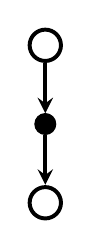
\begin{tikzpicture}


  % TD 1 step
  \node[draw,circle,scale=1.2, fill=white, line width=0.5mm] (s_0) at (0,0) {};
  \foreach \xa in {-1} {
      \node[draw,circle,fill,scale=0.8] (b0\xa) at (0, \xa) {};
      \node[draw,circle,scale=1.2, fill=white,line width=0.5mm] (s0\xa) at (0,\xa-1) {};
      \draw[-stealth, line width=0.5mm] (b0\xa) -- (s0\xa);
  }
  \draw[-stealth, line width=0.5mm] (s_0) -- (b0-1);

\end{tikzpicture}
\end{document}